\problemname{Bottle Flip}

\newcommand{\maxd}{1000}

\illustration{.25}{bottles}{Three bottles with different amounts of water.}% Source: Own work
It marks the year 2022 where the \emph{bottle flip challenge} finally reached the last people on earth; the NWERC Jury.
As you may know, the objective of the challenge is to flip a bottle of water $360^{\circ}$ through the air and hope that it lands standing upright.
Figure~\ref{fig:flip} demonstrates a successful bottle flip.

After many failed attempts, we noticed that this task gets significantly easier if the bottle is filled with just the right amount of water.
The simple reason for this is that the amount of water affects the centre of mass of our bottle as it is about to land.\footnote{
    For the sake of completeness, we define the centre of mass as
    the unique point at which the whole mass of the bottle could be concentrated
    without changing the bottle's reaction to gravity,
    regardless of the orientation of the bottle.
    Note that we implicitly assume that the water will stay at the bottom of the bottle.
    This defines exactly what you would intuitively think of as centre of mass.
}
A lower centre of mass makes it easier for the bottle to stay upright after it lands.
Unfortunately, the optimal amount of water depends on the bottle, and we already wasted enough time on this challenge\dots

\begin{figure}[!h]
	\centering
	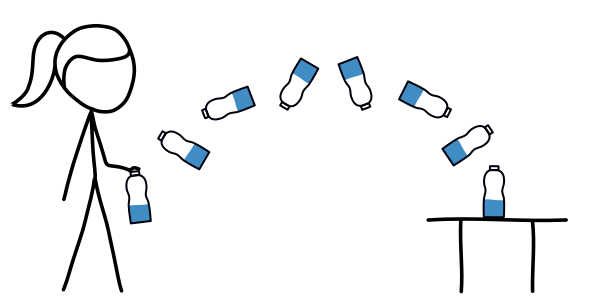
\includegraphics[width=0.47\textwidth]{sketch}
	\caption{Sketch of a bottle flip.
		The bottle is filled to roughly $33\%$ to ease the challenge.}
	\label{fig:flip}
\end{figure}

Given that our bottle is a perfect cylinder of height $h$ and radius $r$,
determine the optimal amount of water the bottle should contain so that our
chances of landing a successful bottle flip are maximised.
You can assume that
both the water and the air contained in the bottle have uniform density, and
that the weight of the bottle itself is negligible.

\begin{Input}
    The input consists of:
    \begin{itemize}
        \item One line with four integers $h$, $r$, $d_a$, and $d_w$ ($1 \leq h, r, d_a, d_w \leq \maxd$, $d_a < d_w$), where $h$ and $r$ are the height and radius of the bottle, and $d_a$ and $d_w$ are the densities of air and water, respectively.
    \end{itemize}
\end{Input}

\begin{Output}
    Output the height such that filling the bottle with water up to this height results in the lowest possible centre of mass while the bottle is standing upright.
    Your answer should have an absolute or relative error of at most $10^{-6}$.
\end{Output}

\pagebreak % Force a page break so that it's easier to see when a single line is rendered on the second page
